%-----------------------------------------------------------------------------------------------------------------
\chapter[Approach]{Approach}
\label{ch:approach}

\cred{\textbf{Thesis part of João Pedro Carvalho de Souza}}

\section{Simulated Annealing applied to Multi-fingered Grasping}

The Simulated Annealing proposed by~\cite{Ciocarlie2009} inserted in \textit{Graspit!} simulator~(\cite{AndrewT2004}) is one of the tools embedded in the grasp pipeline proposed in the present thesis. A brief explanation will be done here, and any further information can be verified on the referred papers.

The \ac{SANN} is a heuristic based on the cooling of a set of atoms to a minimum state of energy, and it was first introduced by~\cite{kirkpatrick1983} in a Statistical Mechanics optimization algorithm application. The ``Very Fast Simulated Re-Annealing'' was an improvement made by Ingber at~\cite{ingber1988} and used here. Since it is based on temperature, Ingber proposed that its cooling process decrease as described by Equation~\ref{eq:temperature}

\begin{equation}
T=T_{0} \cdot exp{(-k^{1/D})}
\label{eq:temperature}
\end{equation}

\noindent
where $D$ is the dimensional search space, $k$ a \ac{SANN} parameter step, and $T_0$ is the \ac{SANN} the initial temperature.

Each algorithm iteration generates new state variables following a rule of neighboring. Considering current and a new variable state as $S_{current}$ and $S_{new}$, this rule yields to Equation~\ref{eq:neighbors}.

\begin{equation}
S_{new}=S_{current}+T \cdot(-1)^{round(Rand(0,1))} \cdot\left(1+\frac{1}{T}\right)^{Rand(-1,1)}
\label{eq:neighbors}
\end{equation}

and the probability to change the state between the current to the new one is defined by Equation~\ref{eq:very_fast_snn_prob} where $Q( \dot )$ represents the objective function of the optimization problem.

\begin{equation}
exp({\frac{Q(S_{current})-Q(S_{new})}{T}})>Rand(0,1)
\label{eq:very_fast_snn_prob}
\end{equation}

Regarding the multi-fingered grasp procedure, the objective function to be optimized by \ac{SANN} is based on the hand posture $\mathbf{p}$ and, the position and orientation of the wrist $\mathbf{w}$ as follow:

\begin{equation}
Q=f(\mathbf{p}, \mathbf{w}), \quad \mathbf{p} \in \mathcal{R}^{d}, w \in \mathcal{R}^{6}
\label{eq:fob_grasp}
\end{equation}

\noindent
where $d$ is the number of intrinsic hand \acp{DOF}.

As discussed by~\cite{Ciocarlie2009}, the hand posture is defined by \textit{eigengrasps}, a subspace of movement based on how human-generated hand postures. The \textit{eigengrasps} reduces the DOFs of the hand based on how humans select appropriate grasps and hand postures. Studies show that humans simplify, unconsciously, the problem with a pattern in the movement. More information can be verified in~\cite{Ciocarlie2009,Santello2002}. The \textit{eigengrasp} ($\mathbf{e}_i$) is defined by hand, and it is a $d$-dimensional direction vector that represents the motion of a group joint space that constitute it. Therefore, a posture can be defined by Equation~\ref{eq:eigengrasp_posture}.

\begin{equation}
p=\mathbf{p}_m+\sum_{i=1}^{b} a_{i} \mathbf{e}_i
\label{eq:eigengrasp_posture}
\end{equation}

\noindent
with posture origin defined by $\mathbf{p}_m$ and $b$ the total number of \textit{eigengrasps}. Since it is a linear combination, the parameter array $\mathbf{a} = [a_0, a_1, ... , a_b]$  will be the optimization variable in the Equation~\ref{eq:fob_grasp} together with the $\mathbf{w}$. Therefore, the dimensional search space $D$ has a reduced length, i.e. $D = sizeof(\mathbf{a}) +  sizeof(\mathbf{w})$.

The optimization algorithm tries to minimize the linear and angular distance of the \ac{ICP} that constitute the \ac{ICR}, see Figure~\ref{fig:icp_opt}. The \ac{ICR} is a contact region model (a predefined group of distributed \acp{ICP}) used to calculate the interaction of the algorithm, thus it is possible to create a feasible procedure.
Therefore, the objective function to be minimized is describe by Equation~\ref{eq:fob_grasp_complete} where $N$ is the number of total contacts in \ac{ICR}, $\mathbf{\hat{n}}_{i}$ is the surface normal, $\mathbf{o}_{i}$ the distance between the \ac{ICP} and the object ($i \in N$). The scalar $\alpha$ is a range adjust factor between the distance and the normalized dot product of the second sum part.    

\begin{figure}[h]\vspace*{0}
\centerline{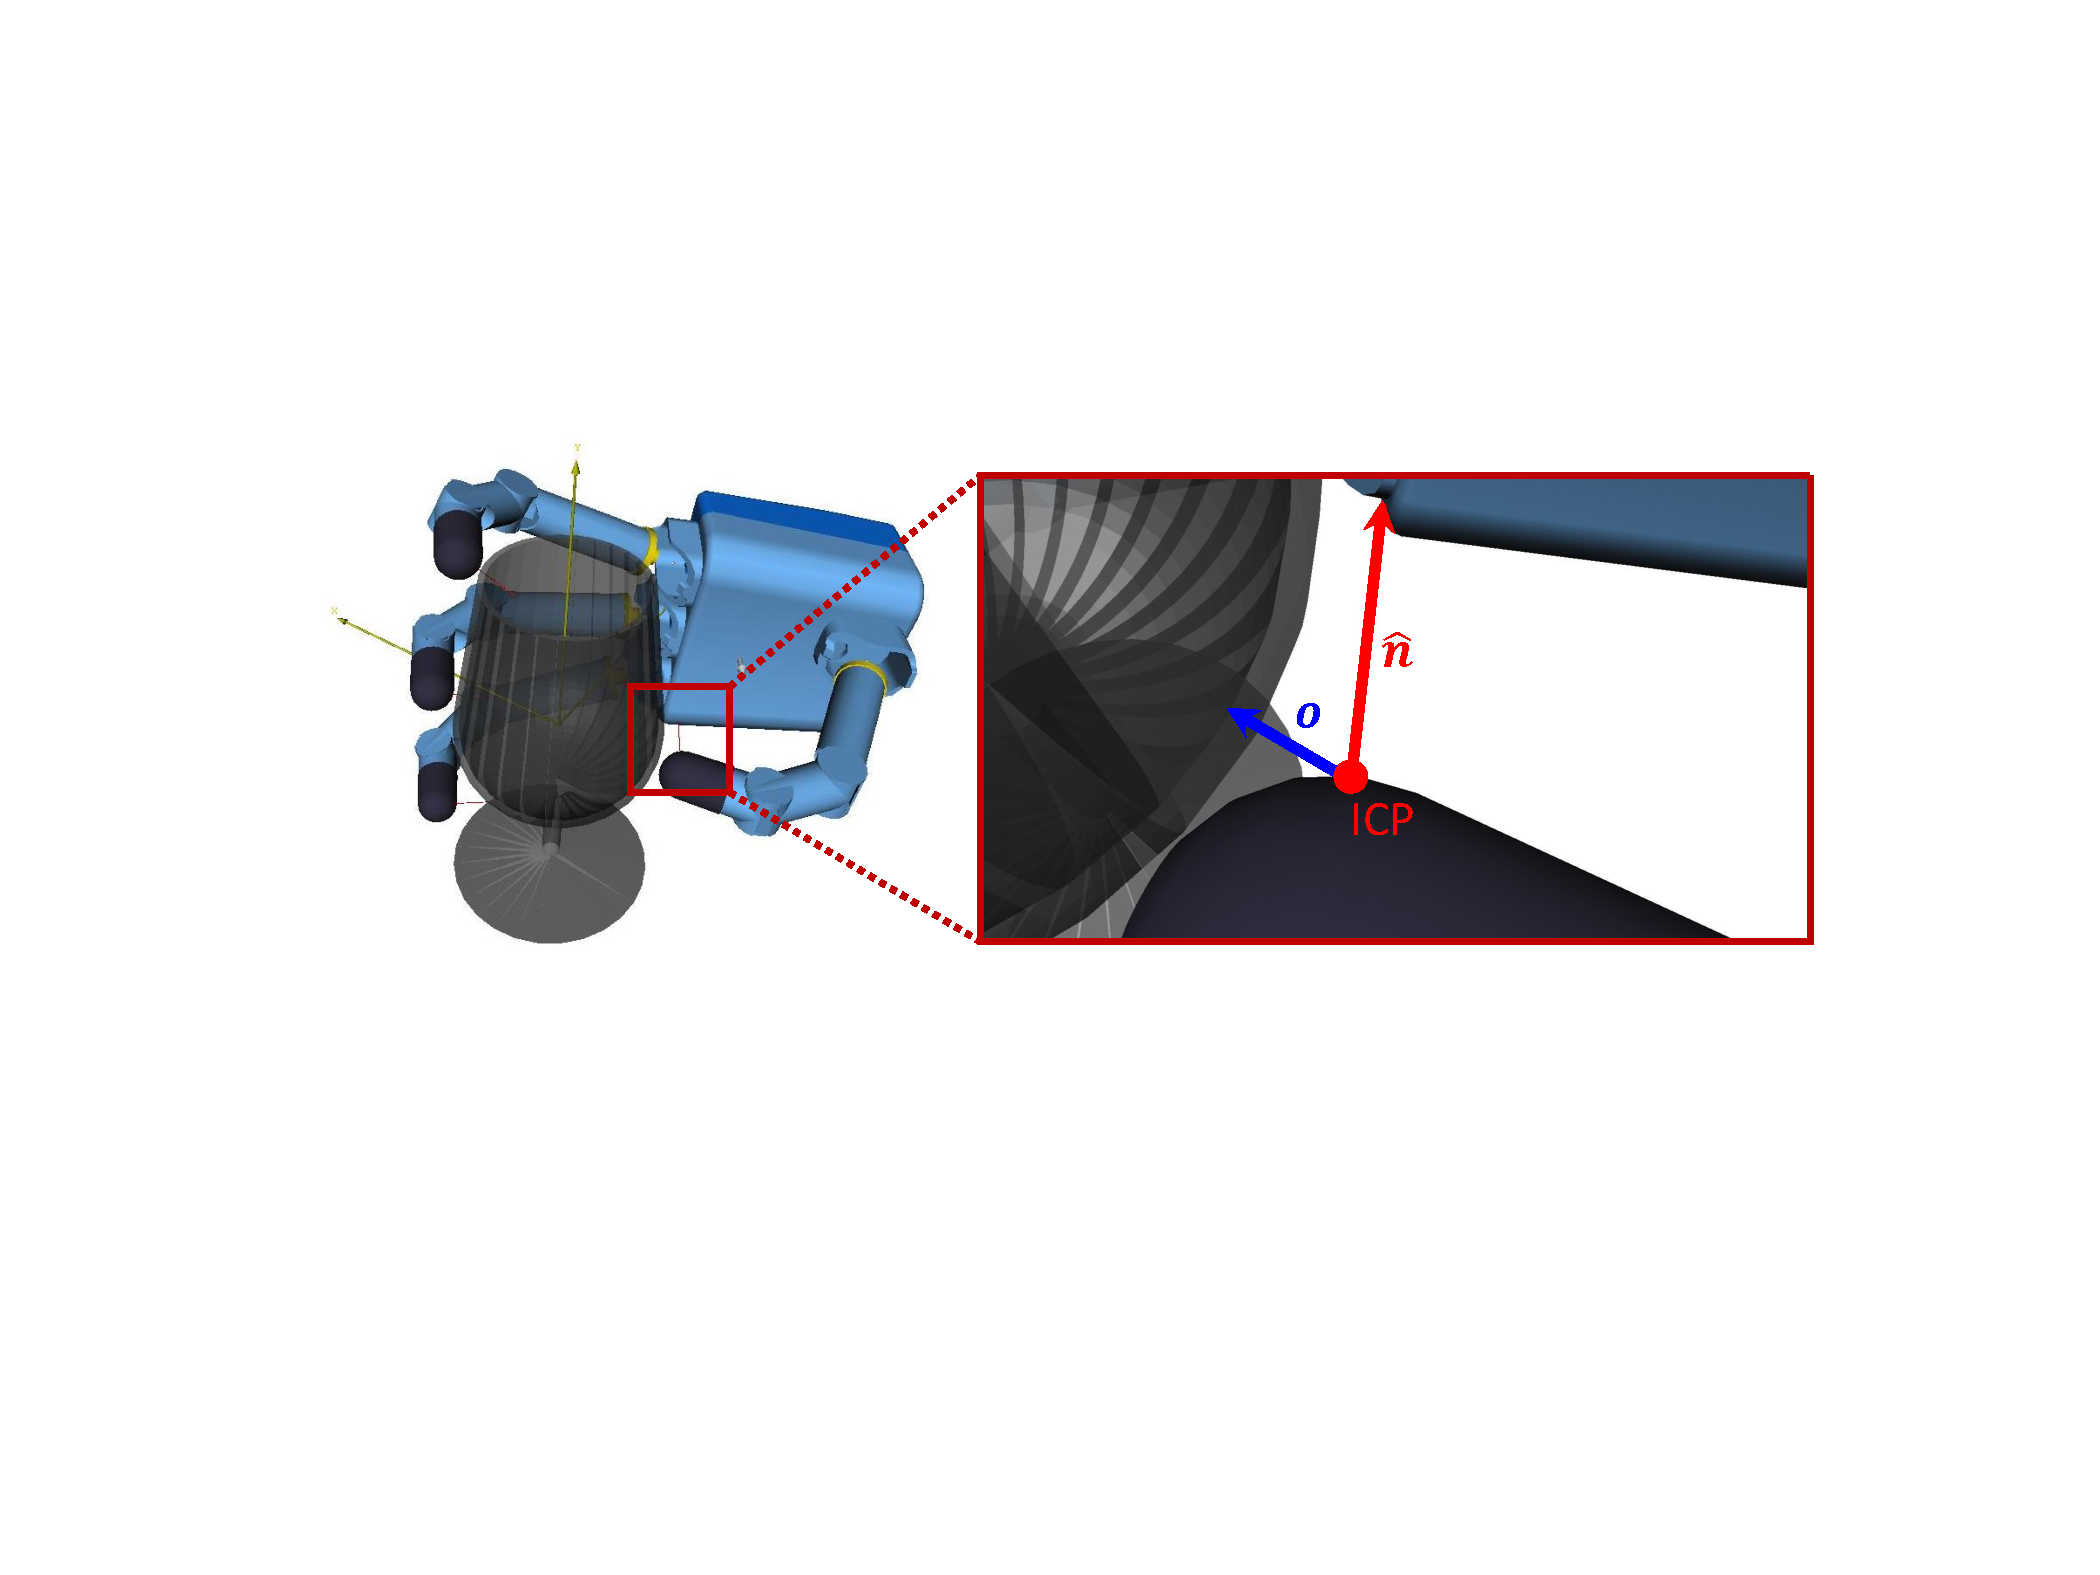
\includegraphics[trim={0cm 0cm 0cm 0cm},clip,width=1\linewidth,angle=0]{Cap4/Figuras/ICPreduction.png}}
\caption{Grasp optimization process elucidation}
\label{fig:icp_opt}
\end{figure}


\begin{equation}
Q=\sum_{i=1}^{N}\left(1-\delta_{i}\right)\hspace{0.5cm}\textnormal{with}\hspace{0.5cm}\delta_{i}=\frac{\left|\mathbf{o}_{i}\right|}{\alpha}+\left(1-\frac{\mathbf{\hat{n}}_{i} \cdot\mathbf{o}_{i}}{\left|\mathbf{o}_{i}\right|}\right)
\label{eq:fob_grasp_complete}
\end{equation}

The algorithm proposed by~\cite{Ciocarlie2009}, and used in this proposal, is replicated in Algorithm~\ref{alg:snn_grasp}.
As already mentioned, the variables that define the states are $\mathbf{a}$, related to the \textit{eigengrasp}, and $\mathbf{w}$, related to the wrist pose. The ``\textit{ObjFunc}'' is described by Equation~\ref{eq:fob_grasp_complete}. The ``\textit{Ngbr}'' is the calculating of neighbouring of the state variables using the Equation~\ref{eq:neighbors} and, ``\textit{Probability}'' is the function to perform the probability of jump to a new state according to Equation~\ref{eq:very_fast_snn_prob}. Since this step of the algorithm is based on \textit{Graspit!}, the ``ForwardKinematics'' and collision check are are parts of this tool.

\begin{algorithm}[]
 \ForAll {variables of CurrentState} 
 {CurrentState.variable = RandomValue()}\EndFor
 QCurrent = ObjFunc(CurrentState)\;
 Iterations = 0\;
 QSaved = 0\;
  \While{Iterations \neq MaxIterations}{
  {Generate a new state as a neighbor of current state}\;
  \Repeat{legalState == true}
  {
    \ForAll{variables of NewState}{
    Sim. Annealing neighbor generation function\;
    NewState.variable = Ngbr(CurrentState.variable)\;
    }\EndFor
    Apply ForwardKinematics(NewState)\;
    \If{collisions detected \textnormal{\textbf{or}} joint limits exceeded} {
     legalState = false\;
    } \Else{
    legalState = true
    }
    \EndIf
  }
  \Until 
  QNew = ObjFunc(NewState)\;
  \If{QNew $>$ QSaved}
  {
    Insert NewState in SavedStatesList\;
    QSaved = lowest ObjFunc value in SavedStateList\;
  }\EndIf
  Sim. Annealing probability of "jumping" to new state\;
  PJump = Probability(QCurrent, QNew)\;
  \If{PJump $>$ 0.5}{
  CurrentState = NewState\;
  QCurrent = QNew\;
  }\EndIf
  Iterations = Iterations + 1\;
  }\EndWhile
  
 \caption{Simulated Annealing applied to grasping}
 \label{alg:snn_grasp}
\end{algorithm}





